% !TeX root = notes.tex

\documentclass{article}
\usepackage[utf8]{inputenc}
\usepackage[english]{babel}
\usepackage{xcolor}
\usepackage{minted}
\usepackage{graphicx}
\usepackage{tikz}

\usepackage[scaled]{helvet}
\renewcommand*\familydefault{\sfdefault}

\usepackage[hmargin=2.54cm, vmargin=2.54cm]{geometry}

% Define custom colours
\definecolor{darkgray}{RGB}{15, 15, 25}
\definecolor{lightgray}{RGB}{200, 200, 215}

\pagecolor{darkgray}
\color{lightgray}

\begin{document}

\begin{titlepage}
    \centering
    \vspace*{2cm} % More space at the top for a balanced look
    
    {\LARGE\bfseries CM1005 - Introduction to Programming I}\\[0.8cm]
    {\large\bfseries BSc Computer Science}\\[0.5cm] % Slightly less space before your name, added bold to program
    
    {\large\textit{Nathan Donovan}}\\[1.5cm] % Less space before the logo to bring elements closer

    
\includegraphics[scale=0.1]{../images/university-of-london-logo.png}\\[1.5cm] % Adjusted scale for visibility
    {\Large\bfseries University of London}\\[1cm] % Bold for the university name for importance
    {\large \today}

    \vfill % This pushes the following text to the bottom
    
    % Optional: Department/Faculty Name Here
    % {\large Department of Computer Science}\\[0.5cm] % Example
    
\end{titlepage}

\newpage
\section{p5.js - JavaScript Library for Creative Coding}
Tools used: p5.js, Brackets.io, JavaScript

\subsection*{p5.js}
\begin{itemize}
    \item Projects / programs must be opened at the folder level in Brackets.io / other IDE for live preview to work.
    \item Work on sketch.js file only. 
        \begin{itemize}
            \item index.html is boilerplate for the sketch to run as a web page.
            \item p5.min.js is the p5.js library code.
        \end{itemize}
\end{itemize}

\vspace*{0.5cm}
\noindent Function used to set up the sketch, width and height are specified in pixels with the origin (0,0) at the top left hand corner of the browser window:

\vspace*{0.25cm}
\begin{minted}{javascript}
    function setup() {
        createCanvas(width, height);
    }
    \end{minted}


\begin{center}
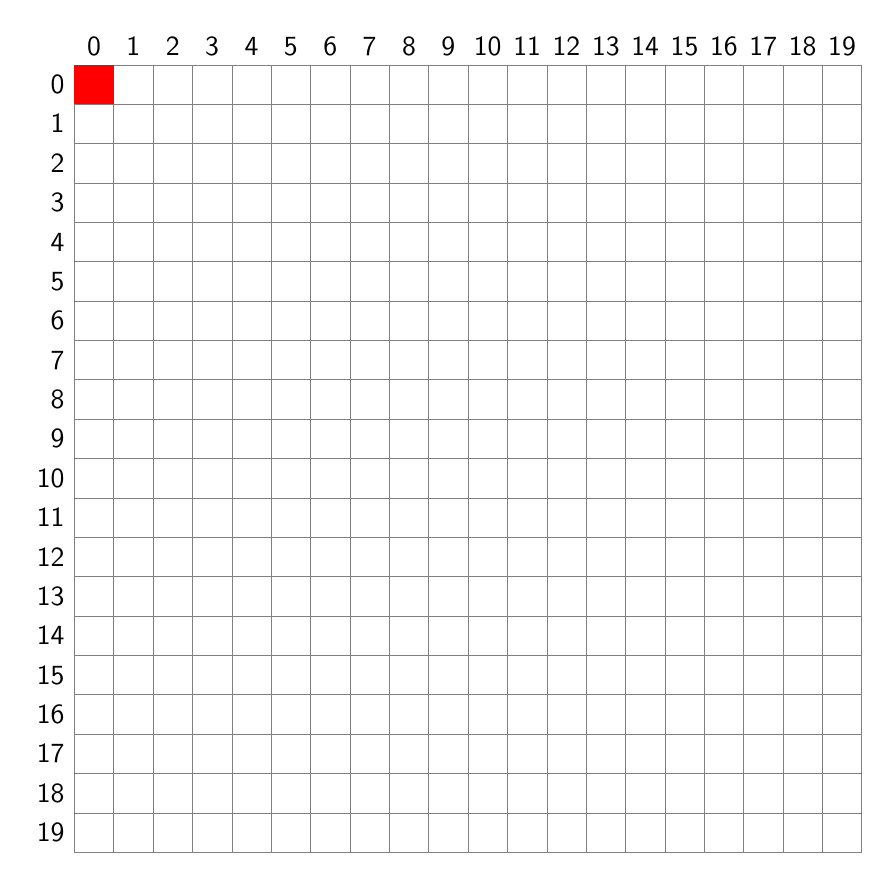
\begin{tikzpicture}[scale=0.50] % Scale to make each "pixel" larger or smaller
    % Draw the 20x20 grid
    \draw[step=1, gray, very thin] (0,0) grid (20,20);
    
    % Highlight the origin (0,0)
    \fill[red] (0,19) rectangle (1,20);

    % Loop for labels on the left axis
    \foreach \y in {0,...,19}
        \node[left] at (0,19.5-\y) {\y};
    
    % Loop for labels on the top axis
    \foreach \x in {0,...,19}
        \node[above] at (\x+0.5,20) {\x};   
\end{tikzpicture}

\vspace*{0.5cm}
Origin pixel highlighted in red at (0, 0), example canvas is 20 x 20 pixels.
\end{center}

\newpage
\noindent Function used to contain the drawing commands in the sketch:
\begin{minted}{javascript}
    function draw() {
        // Various commands available as part of the p5.js library
    }
    \end{minted}

\end{document}
